% =====================================================================
%  Group-Fair Stochastic Gradient Descent via Masked Optimal Transport
%  ICASSP submission -- 4 pages + 1 page references
%
%  Compile:  pdflatex main ; pdflatex main
%  Replace the local stand-in spconf.sty with the official ICASSP one
%  before submitting. Nothing in this file needs to change.
%
%  Markers you should sweep before submission:
%     %%FILLIN   -- a number or description only you can supply
%     %%CHECK    -- a claim worth re-reading against the code
% =====================================================================
\documentclass{article}
\usepackage{spconf,amsmath,amssymb,amsthm,graphicx,booktabs,multirow}
\usepackage{algorithm}
\usepackage{algpseudocode}
\usepackage[usenames,dvipsnames]{xcolor}
\usepackage{url}
\usepackage{tikz}
\usetikzlibrary{positioning,arrows.meta,fit,backgrounds}

% ---------------------------------------------------------------- macros
\newtheorem{theorem}{Theorem}
\newtheorem{lemma}[theorem]{Lemma}
\newtheorem{proposition}[theorem]{Proposition}
\newtheorem{corollary}[theorem]{Corollary}
\theoremstyle{definition}
\newtheorem{assumption}[theorem]{Assumption}
\newtheorem{remark}[theorem]{Remark}

\newcommand{\R}{\mathbb{R}}
\newcommand{\E}{\mathbb{E}}
\newcommand{\PP}{\mathbb{P}}
\newcommand{\Nn}[1]{[#1]}
\newcommand{\simplex}[1]{\Delta^{#1-1}}
\newcommand{\CVaR}{\mathrm{CVaR}}
\newcommand{\KL}{\mathrm{KL}}
\newcommand{\Proj}{\Pi_{\mathcal{C}}}
\newcommand{\avot}{\textsf{GAVOT}}
\newcommand{\avotcvar}{\textsf{GAVOT+CVaR}}
\DeclareMathOperator*{\argmin}{arg\,min}
\DeclareMathOperator*{\argmax}{arg\,max}

\newcommand{\best}[1]{\textbf{#1}}

% ---------------------------------------------------------------- title
\title{Group-Fair Stochastic Gradient Descent \\ via Masked Optimal Transport}

\name{Herlock (SeyedAbolfazl) Rahimi \qquad Dionysis Kalogerias%
\thanks{This work is supported by NSF under Grant 2242215.}}
\address{Department of Electrical and Computer Engineering, Yale University, New Haven, CT, USA\\
\texttt{\{herlock.rahimi, dionysis.kalogerias\}@yale.edu}}

\begin{document}
\ninept
\maketitle

\begin{abstract}
Minibatch SGD is group-blind. Which groups appear in a batch is decided by how
often they occur in the data, not by how much they are meant to count in the
objective, and when the two disagree the iterates converge to a
prevalence-weighted surrogate rather than to the target risk. The gap is a bias,
so no amount of training removes it. A minibatch is a partial-participation
event over groups, which makes group-fair training an instance of federated
aggregation under availability skew, and we carry the masked optimal transport
construction of \textsf{FedAVOT} across. Aligning the
batch-composition distribution $q$ with the target importance distribution $p$
produces per-batch group weights whose induced stochastic subgradient is exactly
unbiased for the target risk, giving the standard $O(1/\sqrt{T})$ rate in the
nonsmooth convex regime with a constant that does not depend on how many groups
a batch happens to cover. Exact alignment is feasible precisely under a Hall-type condition, which reduces
to the per-group requirement that importance not exceed observation rate; past
it Sinkhorn returns an information projection and a residual we compute in
closed form rather than bound. That closed form turns the excess risk into two
terms, an alignment gain fixed by the instance and an optimization residual paid
by the estimator, and a severity sweep over eleven availability skews on Adult
and IMDb-Wiki shows the two crossing: transport wins while the gain exceeds the
residual and loses past it, at a threshold the decomposition locates in advance.
The residual is a stepsize artifact, not a property of the method, and a
decaying schedule removes it on every instance where it had reversed the sign.
A mean--CVaR layer composed on top reaches the worst group at rate
$O(\kappa(\alpha,\gamma)/\sqrt{T})$.
\end{abstract}

\begin{keywords}
Group fairness, optimal transport, stochastic gradient descent,
distribution shift, conditional value at risk.
\end{keywords}

% =====================================================================
\section{Introduction}
% =====================================================================

A classifier is rarely asked to minimize one risk. It is asked to minimize one
while behaving acceptably on subpopulations the training distribution
under-represents: a diagnostic model across patient groups, a recognition system
across demographic strata \cite{buolamwini2018gender,hashimoto2018repeated,%
sagawa2020dro}. The standard response is to change the objective, replacing the
empirical risk by $F_p(\theta)=\sum_i p_i f_i(\theta)$ with $p$ the weighting
one actually wants, uniform, inverse to prevalence, or externally dictated
\cite{mohri2019agnostic,li2020fair}.

This paper is about a gap between writing that objective down and optimizing it.
Minibatch SGD does not see $p$: it sees a batch, whose group composition is
governed by prevalence and by the sampler, so averaging the per-example
gradients descends a different function. The estimator is not merely noisy, it
is biased, by a fixed vector that survives $T\to\infty$ and any stepsize
schedule. Rebalancing the sampler is the usual and only partial fix: a group
whose prevalence is below the resolution of the batch size cannot be sampled
into every batch however the sampler is tilted, and upscaling the few examples
that do appear reintroduces an amplitude distortion that destabilizes the
iterates \cite{rahimi2025fedavot}.

\noindent\textbf{Groups as clients.}
The same mismatch is the central object of a different literature. In federated
learning the \emph{availability distribution} $q$ over which clients participate
in a round rarely matches the \emph{importance distribution} $p$ that defines
the objective, and \textsf{FedAvg} consequently optimizes a surrogate whose
weights are induced by the availability process rather than chosen
\cite{rahimi2025agnostic,wang2020objective,cho2022biased}. \textsf{FedAVOT}
\cite{rahimi2025fedavot} removes that mismatch by posing aggregation as a masked
optimal transport (MOT) problem: find a coupling whose column marginal is the
availability law and whose row marginal is the target $p$, supported only on
client-round pairs that actually occurred. The observation driving this paper is that a minibatch is a participation
event: the groups represented in $B^t$ are the active set $S^t$, its law is $q$,
and the weighting one wants is $p$. Group-fair SGD is federated aggregation with
the federation collapsed onto one machine. We call the method \avot{} and keep
the \textsf{FedAVOT} label in figures, the aggregation rule being unchanged.

\noindent\textbf{Contributions.}
\begin{enumerate}\itemsep0pt\parskip0pt\topsep2pt
\item \emph{The reduction} (Sec.~\ref{sec:setup}). Group-blind minibatch SGD reduces, under
uniform-within-batch averaging, to agnostic \textsf{FedAvg} with one local step, so the surrogate identity of
\cite{rahimi2025agnostic} names the function SGD actually minimizes, and
transport weights make the batch subgradient exactly unbiased for $\nabla F_p$
(Lemma~\ref{lem:unbiased}).
\item \emph{A coverage law and a severity measure} (Cor.~\ref{cor:batchsize}).
Feasibility is Hall-type and reduces on singletons to $p_i\le r_i$, importance
below observation rate, so the \emph{infeasible mass}
$\nu\triangleq\sum_{i:p_i>r_i}p_i$ is the natural severity axis, computable
before training.
\item \emph{A two-term decomposition that locates the crossover}
(Thm.~\ref{thm:infeasible}, Sec.~\ref{sec:exp}). Past the Hall condition the
excess splits into an \emph{alignment gain} $\Delta_{\mathrm{floor}}$, the
distance between the two optima each rule actually converges to, and an
optimization residual. The gain is exact and instance-fixed; the residual is
paid by the estimator. We sweep eleven skews and watch the two cross.
\item \emph{Risk-averse layer} (Sec.~\ref{sec:cvar}). Mean--CVaR over groups
composes with the transport weights without disturbing unbiasedness, at rate
$O(\kappa(\alpha,\gamma)/\sqrt{T})$,
$\kappa(\alpha,\gamma)=\gamma+(1-\gamma)/\alpha$.
\end{enumerate}

\noindent\textbf{Related work.}
Reduction methods for group fairness return randomized mixtures or carry an
approximation constant tied to a fixed class
\cite{agarwal2018reductions,cotter2019twoplayer,chamon2020pacc}.
Distributionally robust and worst-group objectives
\cite{sagawa2020dro,hashimoto2018repeated,levy2020large} change the functional
rather than the sampler and are complementary: our CVaR layer is one such
functional, obtained on top of transport rather than instead of it. Importance
sampling for SGD \cite{rizk2021importance,katharopoulos2018not} corrects
variance, not the identity of the minimized objective.

% =====================================================================
%  Section 2: Problem Formulation  (replaces "Group-Blind SGD and its
%  Surrogate" in main.tex; all labels kept so the rest of the paper
%  resolves unchanged).  Structure follows FedAVOT Sec. 1 and CAMSAP
%  Sec. 2: objective, sampling model, surrogate identity, the question.
% =====================================================================
\section{Problem Formulation}
\label{sec:setup}
% =====================================================================

\noindent\textbf{Groups and objectives.}
Let $\mathcal{X}\subseteq\R^d$ be a feature space and $\mathcal{Y}$ a label
space, and let the population be partitioned into $N$ groups indexed by
$i\in\Nn{N}$ (demographic categories, devices, environments) with
\emph{prevalences} $\pi\in\simplex{N}$, $\pi_i=\PP[\text{group }i]$. Group $i$
carries a distribution $\mathcal{D}_i$ on $\mathcal{X}\times\mathcal{Y}$ and
the risk
\[
f_i(\theta)\;\triangleq\;\E_{(X,Y)\sim\mathcal{D}_i}\big[\ell(m(X;\theta),Y)\big],
\qquad \theta\in\mathcal{C}\subseteq\R^{d'},
\]
where $m(\cdot\,;\theta)$ is the predictor and $\ell$ the loss. Empirical risk
minimization weights the groups by prevalence, $F_\pi=\sum_i\pi_i f_i$, and a
majority group therefore dominates the trained model. The remedy is to fix an
\emph{importance distribution} $p\in\simplex{N}$ and minimize
\begin{equation}
F_p(\theta)\;\triangleq\;\sum_{i=1}^{N}p_i f_i(\theta),
\qquad
\theta^\star\in\argmin_{\theta\in\mathcal{C}}F_p(\theta).
\label{eq:target}
\end{equation}
Uniform $p$ is the category-uniform objective, $p_i\propto 1/\pi_i$ the
inverse-prevalence one, and $p$ may equally encode a fairness constraint or
be imposed externally \cite{mohri2019agnostic,li2020fair}. Throughout,
\begin{assumption}
\label{ass:std}
$\mathcal{C}$ is convex and compact with diameter $D$; each $f_i$ is convex on
$\mathcal{C}$ and $0\le f_i\le M$; and every stochastic subgradient
$g_i(\theta)$ of $f_i$ returned by the sampler satisfies
$\E\|g_i(\theta)\|^2\le G^2$ on $\mathcal{C}$.
\end{assumption}
\noindent These are the assumptions of \cite{rahimi2025agnostic,rahimi2025fedavot}
restated for groups; they place no restriction on $p$ or on $\pi$.

\noindent\textbf{Prevalence versus importance.}
Minibatch SGD does not see $p$. At step $t$ the sampler draws a batch $B^t$ of
$b$ examples; write
\[
A^t\;\triangleq\;\{\,i\in\Nn{N}: B^t\ \text{contains an example from group }i\,\}
\]
for the \emph{active set} of groups, let $\{A_j\}_{j\in\Nn{M}}$ enumerate its
support, and let $q_j\triangleq\PP[A^t=A_j]$ be the \emph{composition law}.
The observation rate of group $i$ is $r_i\triangleq\PP[i\in A^t]=\sum_{j:\,i\in A_j}q_j$;
under i.i.d.\ sampling $r_i=1-(1-\pi_i)^b$, so a group whose prevalence is
below the resolution of the batch is absent from most batches whatever $p$
says. This is federated learning under partial participation: $A^t$ is the set
of participating clients, $q$ the availability distribution, $p$ the
importance distribution \cite{rahimi2025fedavot,rahimi2025agnostic}. We treat
$q$ as known; otherwise it is estimated offline by simulating the sampler, as
in our experiments.

\noindent\textbf{What group-blind SGD minimizes.}
The group-blind update averages the per-example subgradients of $B^t$, which
assigns group $i\in A^t$ the weight $\widehat{\pi}^t_i$, its share of the
batch, and assigns absent groups zero. Averaging first over the batch given
$A^t$ and then over $A^t\sim q$ is the hierarchical experiment of
\cite[Eq.~4]{rahimi2025agnostic}, and it names the function SGD is in fact
minimizing.

\begin{proposition}[Surrogate objective]
\label{prop:surrogate}
Under Assumption~\ref{ass:std}, group-blind minibatch SGD is a stochastic
subgradient method on $F_{\tilde p}$ with
\begin{equation}
\tilde p_i\;=\;\sum_{j:\,i\in A_j} q_j\,\E\big[\widehat{\pi}^t_i\,\big|\,A^t=A_j\big],
\label{eq:ptilde}
\end{equation}
a probability vector. For i.i.d.\ sampling $\tilde p=\pi$; for uniform
weighting within the batch $\tilde p_i=\sum_{j:\,i\in A_j}q_j/|A_j|$, the
surrogate of agnostic \textsf{FedAvg} \cite[Eq.~2]{rahimi2025fedavot}.
Consequently, for every $\theta\in\mathcal{C}$,
\begin{equation}
\big|F_p(\theta)-F_{\tilde p}(\theta)\big|\;\le\;M\|p-\tilde p\|_1 ,
\label{eq:surrogate-gap}
\end{equation}
and any method that minimizes $F_{\tilde p}$ exactly incurs the excess
$F_p(\theta^\star_{\tilde p})-F_p(\theta^\star)\le 2M\|p-\tilde p\|_1$ on
\eqref{eq:target}, which does not vanish with $T$.
\end{proposition}
\begin{proof}
Conditionally on $A^t=A_j$ the within-group averages are unbiased for
$\partial f_i$, so
$\E[\text{batch subgradient}\mid A^t=A_j]=\sum_{i\in A_j}\E[\widehat\pi^t_i\mid A_j]\,\partial f_i(\theta)$;
averaging over $q$ gives $\sum_i\tilde p_i\,\partial f_i=\partial F_{\tilde p}$,
and $\sum_i\tilde p_i=\sum_j q_j\sum_{i\in A_j}\E[\widehat\pi^t_i\mid A_j]=1$.
Both bounds follow from $0\le f_i\le M$ and the two-point inequality
$F_p(\theta^\star_{\tilde p})-F_p(\theta^\star)\le
[F_p-F_{\tilde p}](\theta^\star_{\tilde p})+[F_{\tilde p}-F_p](\theta^\star)$.
\end{proof}

Proposition~\ref{prop:surrogate} says that the choice of $p$ in
\eqref{eq:target} is decorative unless the aggregation step is changed: the
iterates converge, at the usual rate, to the minimizer of a function whose
weights are induced by the sampler rather than chosen, and the bias
$p-\tilde p$ survives every stepsize schedule. Rebalancing the sampler is
only a partial fix: $\tilde p_i\le r_i$ always, so a group with $p_i>r_i$
cannot be sampled into enough batches however the sampler is tilted, while
upscaling the examples that do appear reintroduces an amplitude distortion
that destabilizes the iterates \cite{rahimi2025fedavot}. The question is the
one posed for federated aggregation in \cite{rahimi2025fedavot}, read on
batches:
\begin{center}
\emph{Can the per-batch group weights be chosen so that SGD driven by the
composition law $q$ converges for the objective defined by $p$?}
\end{center}
The next section answers it, and characterizes exactly when the answer is yes.

% =====================================================================
%  Section 3: Proposed Approach  (replaces "Alignment by Masked Optimal
%  Transport" in main.tex; all labels kept).  Structure follows FedAVOT
%  Sec. 2-3: coupling, feasibility (Hall/flow), Sinkhorn, algorithm,
%  unbiasedness, second moment, rate, infeasible regime.
% =====================================================================
\section{Proposed Approach: Alignment by Masked Optimal Transport}
\label{sec:gavot}
% =====================================================================

\noindent\textbf{Weights as a coupling.}
Let $Y[i,j]\ge 0$ be the weight assigned to group $i$ when the active set is
$A_j$, with $Y[i,j]=0$ for $i\notin A_j$, and let $T[i,j]\triangleq q_jY[i,j]$
be the joint mass carried from composition $j$ to group $i$. Requiring that
the weights be a probability vector on each realized composition, and that
each group receive in expectation the mass $p$ assigns it, is the
\emph{masked optimal transport} (MOT) feasibility problem of
\cite{rahimi2025fedavot},
\begin{equation}
T\mathbf{1}_M=p,\qquad \mathbf{1}_N^\top T=q,\qquad T\ge 0,
\qquad \mathrm{supp}(T)\subseteq E,
\label{eq:mot}
\end{equation}
with mask $E=\{(i,j): i\in A_j\}$ encoding that a group absent from the batch
cannot be weighted. Unlike classical transport
\cite{villani2009,peyre2019} there is no cost to minimize: any coupling
respecting \eqref{eq:mot} serves, and \eqref{eq:mot} is the Kantorovich
problem with the indicator cost $C[i,j]=\infty$ off $E$. Fig.~\ref{fig:mask}
is the picture.

\begin{figure}[t]
\centering
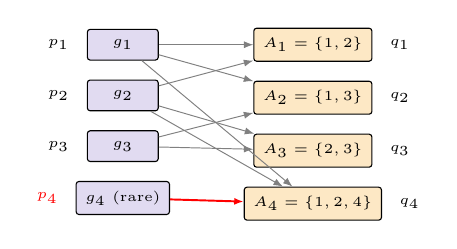
\begin{tikzpicture}[
   node distance=2.4mm,
   grp/.style={draw,rounded corners=1pt,minimum width=9mm,minimum height=3.9mm,font=\tiny,fill=Periwinkle!20},
   atm/.style={draw,rounded corners=1pt,minimum width=13mm,minimum height=3.9mm,font=\tiny,fill=YellowOrange!20},
   e/.style={-{Latex[length=1.2mm]},gray,line width=.35pt},
   lbl/.style={font=\tiny\itshape}
]
\node[grp] (g1) {$g_1$};
\node[grp,below=of g1] (g2) {$g_2$};
\node[grp,below=of g2] (g3) {$g_3$};
\node[grp,below=of g3] (g4) {$g_4$ \tiny(rare)};

\node[atm,right=12mm of g1] (a1) {$A_1=\{1,2\}$};
\node[atm,below=of a1] (a2) {$A_2=\{1,3\}$};
\node[atm,below=of a2] (a3) {$A_3=\{2,3\}$};
\node[atm,below=of a3] (a4) {$A_4=\{1,2,4\}$};

\draw[e] (g1)--(a1); \draw[e] (g2)--(a1);
\draw[e] (g1)--(a2); \draw[e] (g3)--(a2);
\draw[e] (g2)--(a3); \draw[e] (g3)--(a3);
\draw[e] (g1)--(a4); \draw[e] (g2)--(a4); \draw[e,Red,line width=.7pt] (g4)--(a4);

\node[lbl,left=1mm of g1] {$p_1$};
\node[lbl,left=1mm of g2] {$p_2$};
\node[lbl,left=1mm of g3] {$p_3$};
\node[lbl,left=1mm of g4,Red] {$p_4$};
\node[lbl,right=1mm of a1] {$q_1$};
\node[lbl,right=1mm of a2] {$q_2$};
\node[lbl,right=1mm of a3] {$q_3$};
\node[lbl,right=1mm of a4] {$q_4$};
\end{tikzpicture}
\caption{The mask $E$. Batch compositions carry the mass $q$ they occur with;
groups must receive the mass $p$ the objective assigns them. Group $4$ is
reachable only through $A_4$, so exact alignment requires $p_4\le q_4$: the
Hall condition of Thm.~\ref{thm:feas} read on the singleton $I=\{4\}$. Shrinking
the batch deletes $A_4$ from the support and makes $p_4$ unreachable.}
\label{fig:mask}
\end{figure}

\noindent\textbf{When alignment is possible.}
Existence of a coupling is a supply--demand question on the bipartite graph
$E$, and is settled by flow duality.

\begin{theorem}[Feasibility, {\cite[Thm.~1]{rahimi2025fedavot}}]
\label{thm:feas}
For $I\subseteq\Nn{N}$ let $\mathcal{N}(I)=\{j:\exists\,i\in I,\ (i,j)\in E\}$
and $\mathcal{S}(I)=\{j: A_j\subseteq I\}$. Problem \eqref{eq:mot} is feasible
if and only if
\begin{equation}
\sum_{j\in\mathcal{S}(I)}q_j\;\le\;\sum_{i\in I}p_i\;\le\;\sum_{j\in\mathcal{N}(I)}q_j
\qquad\forall\,I\subseteq\Nn{N}.
\label{eq:hall}
\end{equation}
\end{theorem}
Proofs are in the appendix. Read on singletons, \eqref{eq:hall} becomes a
statement one can act on before training starts.

\begin{corollary}[Coverage law and severity]
\label{cor:batchsize}
Feasibility of \eqref{eq:mot} requires $\PP[A^t=\{i\}]\le p_i\le r_i$ for every
$i$, with $r_i=\PP[i\in A^t]$ the observation rate of Sec.~\ref{sec:setup}.
Writing
\begin{equation}
\nu\;\triangleq\!\!\sum_{i\,:\,p_i>r_i}\!\! p_i
\label{eq:batchlaw}
\end{equation}
for the \emph{infeasible mass}, $\nu=0$ iff the upper constraints hold.
Under i.i.d.\ sampling of $b$ examples the upper constraint reads
$b\ge\log(1-p_i)/\log(1-\pi_i)$; under $K$-of-$N$ uniform group sampling it
reads $p_i\le K/N$.
\end{corollary}
\noindent\textbf{Severity.}
Importance may not exceed observation rate: a rare group is reachable only
if the batch is large enough to contain it often enough. The infeasible mass
$\nu$ is the axis we sweep: at $\nu=0$ exact alignment is available, and as
$\nu$ grows more of $p$ sits outside the set of row marginals the mask can
reach. A \emph{feasible} and an \emph{infeasible} regime are two points on
this continuum, and Sec.~\ref{sec:exp} sweeps it instead.

\noindent\textbf{Computing the plan.}
Given feasibility, a coupling is obtained by iterative proportional fitting
(Sinkhorn scaling) on the masked support
\cite{sinkhorn1967,cuturi2013,peyre2019}: starting from any $T^{(0)}>0$ on
$E$ with $\mathbf{1}^\top T^{(0)}=q$, alternate
\begin{equation}
T\leftarrow\mathrm{diag}\big(p\oslash T\mathbf{1}\big)\,T,\qquad
T\leftarrow T\,\mathrm{diag}\big(q\oslash T^\top\mathbf{1}\big)
\label{eq:ipfp}
\end{equation}
until $\|T\mathbf{1}-p\|_1\le\varepsilon$. Each sweep costs $O(|E|)$ with
$|E|\le NM$ and $M$ the number of \emph{realized} compositions rather than
$2^N$; the plan is computed once, offline, and the training loop adds one
lookup and one multiply per group per step. Under \eqref{eq:hall} the
iteration converges to a solution of \eqref{eq:mot}
\cite{sinkhorn1967,csiszar1975}, being block-coordinate ascent on the dual of
the entropic problem $\min\{\sum_E T\log T:\ T\mathbf{1}=p,\ \mathbf{1}^\top T=q\}$.
Since $\mathbf{1}_N^\top T=q$ and $Y=T\mathrm{diag}(q)^{-1}$, every column
$Y[\cdot,j]$ is a probability vector on $A_j$, the property each bound below
uses. Algorithm~\ref{alg:gavot} is the resulting method; $\gamma=1$ is the
risk-neutral rule analyzed here and $\gamma<1$ the risk-averse layer of
Sec.~\ref{sec:cvar}.

\begin{algorithm}[t]
\caption{\avot{}: group-fair SGD by masked transport}
\label{alg:gavot}
\begin{algorithmic}[1]
\Require target $p$, composition law $(q,\{A_j\},E)$, step $\eta$, horizon $T$,
 CVaR parameters $(\alpha,\gamma)$ with $\gamma=1$ for the risk-neutral method
\State $(T,Y)\leftarrow$ Sinkhorn scaling for $(p,q,E)$ \Comment{offline, once}
\State $\theta^0\in\mathcal{C}$, $\ t^0\in\R$
\For{$t=1,\dots,T$}
  \State draw batch $B^t$; set $A^t$, let $j(t)$ be s.t.\ $A_{j(t)}=A^t$
  \State $g^t_i \leftarrow$ stochastic subgradient of $f_i$ from $B^t\cap$ group $i$
  \State $w^t_i \leftarrow Y[i,j(t)]\big(\gamma+\tfrac{1-\gamma}{\alpha}\mathbf{1}\{\hat f^t_i>t^{t-1}\}\big)$
  \State $\theta^{t}\leftarrow\Proj\big(\theta^{t-1}-\eta\sum_{i\in A^t}w^t_i\,g^t_i\big)$
  \State $t^{t}\leftarrow t^{t-1}-\eta(1-\gamma)\big(1-\tfrac{1}{\alpha}\sum_{i\in A^t}Y[i,j(t)]\mathbf{1}\{\hat f^t_i>t^{t-1}\}\big)$
\EndFor
\Ensure $\bar\theta_T=\frac{1}{T}\sum_{t=1}^{T}\theta^t$
\end{algorithmic}
\end{algorithm}

\noindent\textbf{Analysis.}
Everything rests on one identity, \cite[Lem.~1]{rahimi2025fedavot} moved from
model averaging to gradient averaging. Let $g_i(\theta)$ be the stochastic
subgradient of $f_i$ computed from $B^t\cap$ group $i$ and
$\hat g(\theta)=\sum_{i\in A^t}Y[i,j(t)]\,g_i(\theta)$ the transport-weighted
batch subgradient of Algorithm~\ref{alg:gavot}. Transport removes bias; it is
not a variance reduction device.

\begin{lemma}[Unbiasedness]
\label{lem:unbiased}
Let $T$ satisfy \eqref{eq:mot}. Then $\E[\hat g(\theta)\mid\theta]\in\partial F_p(\theta)$
for every $\theta\in\mathcal{C}$.
\end{lemma}
\begin{proof}
Conditionally on $A^t=A_j$, $\E[g_i(\theta)]\in\partial f_i(\theta)$ for
$i\in A_j$. Averaging over $A^t\sim q$,
$\E[\hat g]=\sum_j q_j\sum_{i\in A_j}Y[i,j]\,\partial f_i(\theta)
=\sum_i\big(\sum_j T[i,j]\big)\partial f_i(\theta)=\sum_i p_i\,\partial f_i(\theta)$,
the row-marginal constraint being used in the last step.
\end{proof}

\begin{lemma}[Second moment, free of coverage]
\label{lem:variance}
$\E\|\hat g(\theta)\|^2\le G^2$ for every $\theta\in\mathcal{C}$, with no
dependence on $|A^t|$ or on $N$.
\end{lemma}
\begin{proof}
$Y[\cdot,j]$ is a probability vector on $A_j$, so
$\|\sum_i Y[i,j]g_i\|^2\le\sum_i Y[i,j]\|g_i\|^2$ by convexity of
$\|\cdot\|^2$; take expectations and use $\sum_j T[i,j]=p_i$:
$\E\|\hat g\|^2\le\sum_i p_i\,\E\|g_i\|^2\le G^2$.
\end{proof}

\begin{theorem}[Rate]
\label{thm:rate}
Under Assumption~\ref{ass:std}, if \eqref{eq:mot} is feasible then
Algorithm~\ref{alg:gavot} with $\gamma=1$ and $\eta=D/(G\sqrt{T})$ satisfies
\begin{equation}
\E\big[F_p(\bar\theta_T)\big]-F_p(\theta^\star)\;\le\;\frac{DG}{\sqrt{T}} .
\label{eq:rate}
\end{equation}
\end{theorem}
The constant in \eqref{eq:rate} is that of full-participation SGD and is
independent of how many groups appear in a batch: a composition covering two
groups yields the same bound as one covering all $N$, though with larger
realized variance. The proof uses only the two lemmas and never refers to
$|A^t|$, which is why the rate of \cite{rahimi2025fedavot} transfers verbatim
from aggregation of models to aggregation of gradients.

\noindent\textbf{Outside the feasible region.}
When \eqref{eq:hall} fails, \eqref{eq:mot} has no solution and the iteration
\eqref{eq:ipfp} does not diverge: its iterates accumulate at the coupling
whose row marginal $\hat p\triangleq T\mathbf{1}$ is the KL-closest to $p$
over the reachable polytope
$\mathcal{R}(q,E)=\{T\mathbf{1}:\ T\ge 0,\ \mathbf{1}^\top T=q,\ \mathrm{supp}(T)\subseteq E\}$
\cite{csiszar1975,gietl2013ipfp,peyre2019}. The column marginal is met
exactly, so Lemmas~\ref{lem:unbiased} and~\ref{lem:variance} hold with $p$
replaced by $\hat p$: Algorithm~\ref{alg:gavot} is then unbiased SGD on the
surrogate $F_{\hat p}$, the closest objective the sampler can reach, and the
loss on \eqref{eq:target} is a bias of exactly the shape of
Proposition~\ref{prop:surrogate}. On singletons $\hat p_i\le r_i$, so the
groups with $p_i>r_i$ are truncated at their observation rate and their
missing mass, $\nu$ up to renormalization, is redistributed.

\begin{theorem}[Infeasible regime]
\label{thm:infeasible}
Let $\hat p$ be the row marginal of the Sinkhorn limit,
$\theta^\dagger\in\argmin_{\mathcal{C}}F_{\hat p}$, and write
$\Phi(w)\triangleq F_p\big(\argmin_{\mathcal{C}} F_w\big)$ for the $p$-risk of
the minimizer of the $w$-weighted risk. Then
\begin{equation}
\E\big[F_p(\bar\theta_T)\big]-F_p(\theta^\star)
\;=\;\underbrace{\Phi(\hat p)-\Phi(p)}_{\text{alignment floor}}
\;+\;\underbrace{\varepsilon_T(\hat p)}_{\text{optimization residual}} ,
\label{eq:infeasible}
\end{equation}
where $\varepsilon_T(\hat p)\triangleq\E F_p(\bar\theta_T)-F_p(\theta^\dagger)$
satisfies $\E F_{\hat p}(\bar\theta_T)-F_{\hat p}(\theta^\dagger)\le DG/\sqrt{T}$
and $\varepsilon_T(\hat p)\to 0$ whenever $\bar\theta_T\to\theta^\dagger$.
Group-blind averaging obeys \eqref{eq:infeasible} with $\tilde p$ in place of
$\hat p$. Writing $\Delta_{\mathrm{floor}}\triangleq\Phi(\tilde p)-\Phi(\hat p)$
for the \emph{alignment gain}, transport improves on group-blind averaging
exactly when $\Delta_{\mathrm{floor}}>\varepsilon_T(\hat p)-\varepsilon_T(\tilde p)$,
and every floor is bounded by $\Phi(w)-\Phi(p)\le 2M\|p-w\|_1$.
\end{theorem}
Theorem~\ref{thm:infeasible} replaces the usual bias \emph{bound}
\cite{rahimi2025fedavot} by an exact \emph{decomposition}, both terms of which
are available before training: $\hat p$ and $\tilde p$ from $(p,q,E)$, and
$\Phi$ exactly on instances with a closed-form or convex frontier. The gain is
fixed by the instance and decides the sign of the comparison; the residual is
paid by the estimator and, as Sec.~\ref{sec:exp} shows, is a stepsize
artifact. The $\ell_1$ bound is the weaker object and we report both, because
it turns out too loose to discriminate.


% =====================================================================
\section{A Risk-Averse Layer over Groups}
\label{sec:cvar}
% =====================================================================

Exact alignment delivers the $p$-weighted risk, an average, which can hide a
group. Where the requirement is on the worst group instead, we compose a
mean--CVaR functional over groups on top of the transport weights
\cite{rahimi2025agnostic,rockafellar2000cvar}:
\begin{equation}
F_p^{\alpha,\gamma}(\theta)\;\triangleq\;\gamma F_p(\theta)+(1-\gamma)\,
\CVaR^p_\alpha\big(f(\theta)\big),\quad \alpha,\gamma\in(0,1],
\label{eq:meancvar}
\end{equation}
where $\CVaR^p_\alpha$ is the conditional value at risk of the group-loss vector
under $p$. The Rockafellar--Uryasev representation turns \eqref{eq:meancvar}
into a joint minimization over $(\theta,t)$,
\begin{equation}
\Phi(\theta,t)=\gamma\sum_i p_i f_i(\theta)+(1-\gamma)\Big(t+\tfrac{1}{\alpha}
\sum_i p_i\big[f_i(\theta)-t\big]_+\Big),
\label{eq:ru}
\end{equation}
jointly convex, with subgradients in both arguments again $p$-weighted sums of
per-group quantities, so Lemma~\ref{lem:unbiased} applies unchanged. This is why
the layers compose rather than interfere: transport fixes \emph{which}
distribution the expectation is under, CVaR changes \emph{what} is averaged.
Lines 6 and 8 of Algorithm~\ref{alg:gavot} implement \eqref{eq:ru}.

\begin{theorem}[Rate under mean--CVaR]
\label{thm:cvar}
Under the hypotheses of Theorem~\ref{thm:rate}, Algorithm~\ref{alg:gavot} with
$\eta=\Theta(1/\sqrt{T})$ satisfies
$\E[F_p^{\alpha,\gamma}(\bar\theta_T)]-\min F_p^{\alpha,\gamma}
=O\!\big(\kappa(\alpha,\gamma)/\sqrt{T}\big)$ with
$\kappa(\alpha,\gamma)=\gamma+(1-\gamma)/\alpha$. In the infeasible regime the
bound of Theorem~\ref{thm:infeasible} acquires the same factor on its
statistical term, the bias term being unchanged.
\end{theorem}

Both $\gamma=1$ and $\alpha=1$ recover Theorem~\ref{thm:rate} exactly, so the
grid contains the risk-neutral method along two edges, visible as the constant
row and column of every heatmap below. Sending $\alpha\downarrow 0$ drives
\eqref{eq:meancvar} to the worst group at the cost
$\kappa(\alpha,\gamma)\to\infty$: the parameter prices robustness in the
convergence constant, not in the limit.

\begin{remark}[Relation to constrained learning]
\label{rem:penalty}
$\max_i f_i$ is the exact-penalty limit of $\min f_0$ s.t.\ $f_i\le c_i$, a
fixed price on the largest violation matching penalized and constrained values
once it exceeds the least $\ell_1$ norm on the dual-optimal set
\cite{rahimi2026exactpenalty}. The $\alpha\downarrow 0$ edge of
\eqref{eq:meancvar} is thus the scalarization a constrained specification
selects, with $\kappa$ its price in the rate.
\end{remark}

% =====================================================================
%  Section 5: Experiments  (his verified Sec. 5 plus, from the previous
%  Overleaf: the common protocol, fuller instance descriptions, and the
%  closed-form validation of Theorem thm:infeasible.  Labels kept.)
% =====================================================================
\section{Experiments}
\label{sec:exp}

\noindent\textbf{Instances.}
\emph{Adult} income classification \cite{uci_adult}: logistic regression
($d{=}109$ with intercept, cross-entropy, $\eta{=}0.1$) on $100$
race-homogeneous groups of $30$ samples, the number of groups per race
proportional to its prevalence (White/Black/Asian-Pac./Amer-Ind./Other
$=85/10/3/1/1$); the importance target is the fairness target itself, $1/5$
per race divided equally among its groups, so a group from the smallest
race carries $p_i=0.2$. \emph{IMDb-Wiki} age regression
\cite{rothe2018imdbwiki}: linear regression of age on $128$-d ResNet face
embeddings ($\eta{=}10^{-2}$) over the first $100$ identities with $30$
images, with the cubic importance target $p_i\propto(101-i)^3$.
Observation rates are swept through a one-parameter family: on Adult
$r\propto p^{\beta}$, $\beta\in\{0,\tfrac14,\tfrac12,\tfrac34,1\}$, from
uniform observation (prevalence regime, $\nu{=}.60$: the five groups of the
three smallest races hold $60\%$ of the target against $r_i\approx K/m$)
to importance-aligned ($\nu{=}0$); on IMDb-Wiki $r_i\propto i^{\beta}$,
$\beta\in\{0,\tfrac12,1,\tfrac32,2,3\}$, from uniform observation
($\nu{=}.31$, nine groups) to the mirror image of $p$ ($\nu{=}.88$, $41$
groups), plus the aligned $r_i\propto 101-i$ ($\nu{=}0$). Eleven instances,
$\nu$ from $0$ to $.88$.

\noindent\textbf{Protocol.}
Each step observes $K{=}3$ groups drawn without replacement with
probabilities $\propto r$, which induces $q$ over the $\binom{100}{3}$
compositions; $q$ is estimated from $10^6$ draws of the sampler and the plan
from \eqref{eq:ipfp} on the membership mask, once per instance. Each
observed group takes $H{=}5$ local steps on its own data before the weighted
average, the standard practical deviation from the one-step analysis,
applied to every rule alike since all rules consume the same local updates
from the same draw $A^t$. Rules: \avot{}; \emph{group-blind averaging}, the
uniform average over the observed groups (Proposition~\ref{prop:surrogate}
with $\tilde p_i=r_i/K$); the \emph{fixed multiplier} $m/K$, the rescaling
$(m/K)\,p_i$ that presumes uniform observation; and \emph{full}, every group
every step weighted by $p$, the reference $\Phi(p)$. Stepsize
$\eta_t=\eta/(1+t/1000)$ unless stated, fixed before the comparison and
shared by every rule; across nine schedules (constant, hyperbolic with
$T_0\in\{250,\dots,16000\}$, inverse square root, step, cosine) the winner
never changes on any instance, only the margin does: a faster decay puts
full coverage on its floor and widens the IMDb-Wiki gap (cosine: $84.12$
against $90.69$), a constant stepsize narrows it to a tie. $4000$ steps, $5$
seeds; we report $F_p$ averaged over the last $500$ steps, mean $\pm$ std
over seeds. On both
instances $\argmin F_w$ is available to machine precision (closed form for
least squares, Newton for the logistic loss), so the floors
$\Phi(p),\Phi(\hat p),\Phi(\tilde p)$ of Theorem~\ref{thm:infeasible} are
exact rather than estimated, and in every instance with $\nu=0$ the
iteration \eqref{eq:ipfp} converges to a row error below $3\cdot10^{-8}$,
certifying the remaining inequalities of \eqref{eq:hall}.

% ----------------------------------------------------------- Table 1
\begin{table}[t]
\centering
\caption{Headline cells, tail-500 over $5$ seeds, decaying stepsize. \emph{full}
sees every group every step; \emph{upsamp.}, self-normalized upsampling
(weights $\propto p_i/r_i$ within the batch); LDS, label-distribution
smoothing \cite{yang2021dir}, regression only. The fixed multiplier $m/K$
diverges whenever observation rates are non-uniform.}
\label{tab:overall}
\footnotesize\setlength{\tabcolsep}{2.2pt}
\begin{tabular}{lcccccc}
\toprule
Instance & \avot{} & unif.\ avg & upsamp. & LDS & $m/K$ & full \\
\midrule
Adult, $\nu{=}.60$ & $\best{0.2269}$ & $0.2479$ & $0.2288$ & -- & $0.670$ & $0.2073$ \\
Adult, $\nu{=}0$   & $0.2075$ & $0.2077$ & $0.2075$ & -- & div. & $0.2073$ \\
IMDb, $\nu{=}.31$  & $\best{86.06}$ & $91.63$ & $86.74$ & $94.28$ & $8504$ & $82.95$ \\
IMDb, $\nu{=}0$    & $\best{84.28}$ & $86.37$ & $84.40$ & $89.43$ & div. & $82.95$ \\
\bottomrule
\end{tabular}
\end{table}

% ----------------------------------------------------------- Fig 2
\begin{figure}[t]
\centering
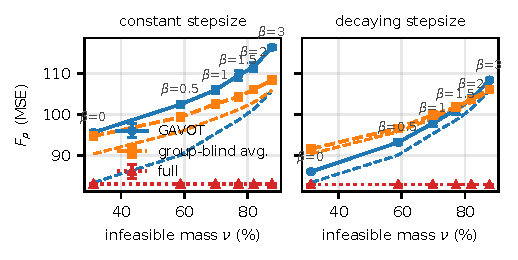
\includegraphics[width=0.92\columnwidth]{figs/severity_imdb.pdf}
\caption{IMDb-Wiki severity sweep. Solid, measured tail-500 ($\pm1$ std);
dashed, the exact floor $\Phi(\cdot)$ each rule converges to. Left, constant
stepsize: the optimization residual swamps the alignment gain and transport
loses everywhere, even where the floors are seven units apart. Right, decaying
stepsize: the residual collapses and the measured curves track their floors, so
transport wins until the floors close at high $\nu$. The sign is set by which of
the two terms of \eqref{eq:infeasible} dominates, not by the regime label.}
\label{fig:severity}
\end{figure}

\begin{figure}[t]
\centering

\includegraphics[width=0.99\columnwidth]{figs/rare_group_adult.pdf}\\[2pt]
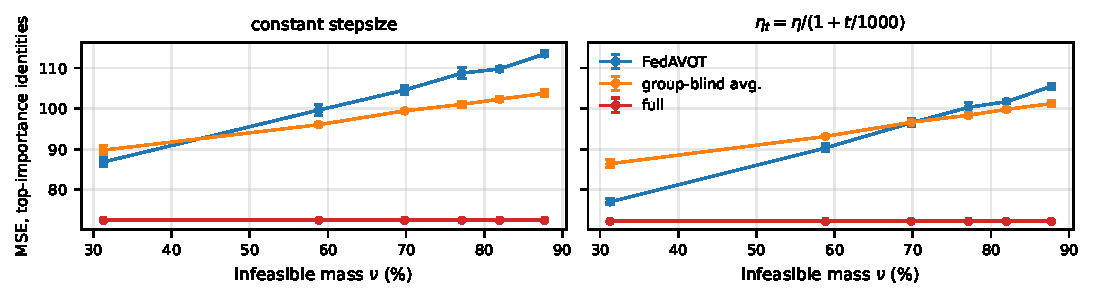
\includegraphics[width=0.99\columnwidth]{figs/rare_group_imdb.pdf}
\caption{Loss on the least represented group, the metric the fairness target
is about. Top, Adult: cross-entropy on race Other, one group of $30$ out of
$100$, to which the category-uniform target assigns $p_i=0.2$; the axis is
the observation-rate exponent, $\beta{=}1$ aligned, $\beta{=}0$ uniform
(prevalence). Bottom, IMDb-Wiki: MSE on the $20$ highest-importance
identities, the least observed ones once $\beta>0$, against $\nu$. Left
panels constant stepsize, right panels decaying. Same protocol as the
tables ($K{=}3$, $H{=}5$, $4000$ steps, tail-500 mean $\pm$ std over $5$
seeds); lower is better. Curves are the group-wise entries of the same runs
as Table~\ref{tab:overall} and Fig.~\ref{fig:severity}.}
\label{fig:rare}
\end{figure}

\noindent\textbf{The least represented group.}
Fig.~\ref{fig:rare} reads the same runs on the group the target exists for.
On Adult, transport lowers the loss on race Other at every skew and under
both stepsizes: $.073$ against $.119$ for group-blind averaging on the
prevalence instance (full coverage $.031$), and $.031$ against $.035$ on the
aligned one, where it matches full coverage. Amer-Indian, the other
single-group race, behaves the same way. On IMDb-Wiki the top-importance
identities show the crossover of Table~\ref{tab:severity} one step earlier:
under decay transport wins at $\nu\le.70$ ($77.0$ against $86.4$ at
$\nu{=}.31$, full $72.2$; $73.6$ against $79.9$ when aligned) and loses at
the three most infeasible skews, while at constant stepsize it wins only at
$\nu{=}.31$. The single most starved group, the one with the largest
$p_i/r_i$ in each instance, sharpens the picture: on Adult it is race Other
itself ($p_i/r_i{=}6.7$); on IMDb-Wiki it is the top identity, where under
decay transport gives $253$ against $331$ at $\nu{=}.31$ and $373$ against
$380$ at $\nu{=}.59$ (full $219$), then loses from $\nu{=}.70$ on, the same
crossover one step earlier still (a $30$-image group, so $\pm5$ to $10$
across seeds). The overall objective and the rare-group loss therefore tell
the same story, with the rare group the more sensitive of the two.

\noindent\textbf{Why transport stops helping.}
The failure is not a bug of the weights; it is the two terms of
\eqref{eq:infeasible} changing sign. A starved group has $p_i>r_i$, so the
plan can deliver at most $r_i$ of its mass: past the coverage law of
Cor.~\ref{cor:batchsize} the reachable target $\hat p$ truncates at the
observation rate, and as $\nu$ grows $\hat p$ and the group-blind $\tilde p$
starve the same groups, so the two floors converge (Table~\ref{tab:severity},
$\Delta_{\mathrm{floor}}$ from $6.99$ to $0.02$). What transport still does
is concentrate weight on the starved group whenever it does appear, $p_i/r_i$
times its batch share, which is exactly the variance Lemma~\ref{lem:variance}
does not see: the second moment is bounded, the variance about the mean is
not, and it is largest on the rare group. Once the floors coincide that
variance is all that separates the two rules, so transport loses by the
residual, by $2$ to $8$ at constant stepsize and by $2.3$ at $\nu{=}.88$ even
under decay. Transport helps exactly while there is mass left to move.

\noindent\textbf{E1: the headline cells.}
Table~\ref{tab:overall} reports the four instances a practitioner would
recognize. Transport wins on three: Adult under prevalence-proportional
availability, $0.2269$ against $0.2479$ ($t{=}45$), and both IMDb cells,
$86.06$ against $91.63$ ($t{=}21$) and $84.28$ against $86.37$ ($t{=}13$). On
Adult with importance-aligned availability the two coincide at the oracle
value, which is what Proposition~\ref{prop:surrogate} predicts when
$\tilde p=p$: there is nothing to correct and transport does not manufacture a
difference. The fixed multiplier diverges on both aligned instances and is far
off on the other two, so naive rescaling is no alternative to solving \eqref{eq:mot}.
Two imbalance baselines sit between the two. Self-normalized upsampling
(weights $\propto p_i/r_i$, renormalized within the batch), the reweighting
form of oversampling rare groups, recovers most of the gain and transport
the rest: $0.2288$ against $0.2269$ on Adult prevalence ($t{=}5.8$) and
$86.74$ against $86.06$ on IMDb skewed ($t{=}2.6$, at the margin of
significance with $5$ seeds); on the aligned instances the two coincide, as
every convex rule must. Downsampling ($\min(p_i/r_i,1)$, normalized) is never
better than upsampling ($0.2308$, $86.90$). Label-distribution smoothing
\cite{yang2021dir}, the standard imbalanced-regression correction, reweights
by the rarity of the label value rather than by how rarely a group is
observed, and trails even group-blind averaging on both IMDb-Wiki instances
($94.28$, $89.43$). On the least represented group the margin of transport
over upsampling widens: $77.0$ against $80.0$ at $\nu{=}.31$ and $73.6$
against $75.6$ when aligned on IMDb-Wiki, $.073$ against $.075$ on Adult
prevalence. Upsampling is the one-shot heuristic for the marginal problem
\eqref{eq:mot} solves exactly, without the feasibility certificate or the
floor decomposition.

% ----------------------------------------------------------- Table 2
\begin{table}[t]
\centering
\caption{IMDb-Wiki severity sweep, decaying stepsize. $\Delta_{\mathrm{floor}}$
is the alignment gain of Theorem~\ref{thm:infeasible}, \emph{gain} the measured
advantage of transport, $t$ its Welch statistic (population std). The excess
residual transport pays averages $1.9$, and the sign flips exactly where
$\Delta_{\mathrm{floor}}$ crosses it. The five Adult skews all sit above their
crossover and are omitted.}
\label{tab:severity}
\setlength{\tabcolsep}{3.0pt}
\begin{tabular}{ccccc}
\toprule
$\beta$ & $\nu$ & $\Delta_{\mathrm{floor}}$ & gain & $t$ \\
\midrule
$0$   & $.31$ & $6.99$ & $\best{+5.57}$ & $20.7$ \\
$0.5$ & $.59$ & $5.71$ & $\best{+3.46}$ & $11.3$ \\
$1.0$ & $.70$ & $3.67$ & $\best{+2.05}$ & $5.4$ \\
$1.5$ & $.77$ & $2.56$ & $+0.58$ & $1.1$ \\
$2.0$ & $.82$ & $1.62$ & $-0.03$ & $-0.1$ \\
$3.0$ & $.88$ & $0.02$ & $-2.28$ & $-7.9$ \\
\bottomrule
\end{tabular}
\end{table}

\noindent\textbf{E2: the crossover, and where the sign comes from.}
Table~\ref{tab:severity} and Fig.~\ref{fig:severity} are the paper's main
evidence. On Adult, whose five skews are omitted from the table, the measured gain tracks
$\Delta_{\mathrm{floor}}$ within $4\%$ at three of five
($.0134$ against $.0129$, $.0050$ against $.0049$, $.0002$ against $.0003$)
and exceeds it at the two most infeasible ($.0210$ against $.0110$, $.0181$
against $.0144$), group-blind averaging sitting further above its floor. On IMDb-Wiki the gain is
uniformly below the floor by an excess optimization residual that is close to
constant in $\beta$, mean $1.9$ in MSE units, and the measured sign flips
precisely where $\Delta_{\mathrm{floor}}$ crosses that value, between
$\beta{=}1.5$ ($2.56$, gain $+0.58$) and $\beta{=}2.0$ ($1.62$, gain $-0.03$).
This is Theorem~\ref{thm:infeasible} read at finite $T$: the sign of the
comparison is a quantity one computes in advance.

\noindent\textbf{E3: the $\ell_1$ bound is too loose to be the criterion.}
The distances $\|p-\hat p\|_1$ and $\|p-\tilde p\|_1$ are also computed on every
instance, and $\|p-\hat p\|_1<\|p-\tilde p\|_1$ holds in all eleven, including
the three where transport loses or ties. The $\ell_1$ form of
Theorem~\ref{thm:infeasible} therefore never predicts a loss and cannot serve as
the criterion; the exact floors can.

\noindent\textbf{E4: the residual is a stepsize artifact.}
The left panel of Fig.~\ref{fig:severity} runs the identical instances at
constant stepsize. There transport loses on all six IMDb skews, by as much as
$7.9$, even at $\nu{=}.31$ where the floors are $6.99$ apart. The transport
weights $Y[\cdot,j]$ concentrate mass on rarely observed groups, so although
Lemma~\ref{lem:variance} bounds the second moment identically for both rules,
the variance about the mean is larger, and at constant stepsize the iterates sit
on a noise floor proportional to it. Under $\eta_t=\eta/(1+t/1000)$ that floor
decays, the measured curves fall onto their dashed floors, and every sign
reversal attributable to the stepsize disappears. The residual is a property of
the schedule, not of the estimator.

\noindent\textbf{E5: the decomposition in closed form.}
The mirrored IMDb-Wiki instance ($\nu{=}.88$) is where
Theorem~\ref{thm:infeasible} can be read off exactly. The Sinkhorn limit
truncates the target at the observation-rate ceiling,
$\hat p_i\approx\min(p_i,r_i)$ up to renormalization (maximum deviation
$.023$), with $\|p-\hat p\|_1=1.58$ of a possible $2$. The frontier is least
squares, so $\Phi(p)=82.9$, matching the measured full plateau $82.95$, and
$\Phi(\hat p)=105.9$: the alignment floor is $23.0$ and the realized bias
equals its exact expression $|(p-\hat p)^\top L(\theta^\dagger)|=30.7$, where
$L$ collects the per-group risks, while the $\ell_1$ form $2M\|p-\hat p\|_1$
is conservative since $M\ge\max_i L_i(\theta^\dagger)\approx 454$.
Group-blind averaging has the same floor to two decimals,
$\Phi(\tilde p)=105.9$: both surrogates starve the same groups, so
$\Delta_{\mathrm{floor}}$ vanishes and the entire measured gap between the
two rules at this endpoint of Table~\ref{tab:severity} is residual, which is
why it is the one instance where transport still loses by a significant
margin under decay ($\beta{=}2$, where the floors are $1.6$ apart, is a tie).

\noindent\textbf{E6: risk aversion, and where it does not help.}
Sweeping $(\alpha,\gamma)$ on a $10\times10$ grid, the overall objective is
minimized on the $\gamma=1$ edge on every instance, which is
$\kappa(1,\gamma)=1$ made visible and confirms that risk aversion costs the
average. The one place the CVaR layer earns its keep is the worst race on Adult
under prevalence availability, where \avotcvar{} at $(0.2,0.7)$ reaches
$0.3624$ against $0.3679$ for \avot{} and $0.3994$ for group-blind averaging.
Per race, transport improves four of five (Black $.179$ vs $.200$, Asian-Pac
$.368$ vs $.399$, Am-Ind $.175$ vs $.189$, Other $.073$ vs $.119$) and regresses
only the majority group ($.339$ vs $.332$), which is what reweighting toward a
category-uniform target is supposed to do.

\noindent\textbf{Why risk aversion does not reach the rare group.}
On the least represented group the CVaR layer never helps: over the whole
$(\alpha,\gamma)$ grid the best rare-group loss is at $\gamma{=}1$, i.e.\ with
the layer switched off, on all four headline instances, and at
$(\alpha,\gamma)=(0.1,0.1)$ it nearly triples the loss on race Other
($.207$ against $.073$) and raises the top-identity loss on IMDb-Wiki from
$77.0$ to $103$. The reason is where the tilt lands. CVaR upweights the
groups whose realized loss exceeds the running threshold, but it can only
tilt among the groups in the batch, and the rare group is absent from most
batches: the extra weight goes to whichever observed group is doing badly
that step, not to the group the target is about. Composed with transport,
the hinge multiplies weights that are already $p_i/r_i$ large, so the
product amplifies the variance of \eqref{eq:infeasible} rather than the
alignment, which is why the loss grows as $\alpha$ shrinks. Risk aversion
changes the functional; it does not change who is observed, and observation
is what the rare group lacks. Transport moves mass toward it whenever it
appears; CVaR cannot, and the one gain it produces, on the worst race above,
comes from tilting among the groups that are present.

% =====================================================================


% =====================================================================
\section{Conclusion}
% =====================================================================

Group-fair training fails in a specific and fixable place: the aggregation step,
blind to the weighting the objective declares. Reading a minibatch as a
partial-participation event makes the fix the masked transport problem that
corrects availability skew in federated learning, with the same feasibility
characterization, an $O(1/\sqrt{T})$ guarantee free of batch coverage, and a
coverage law whose infeasible mass $\nu$ orders instances by severity. Past
feasibility the excess splits cleanly, into an alignment gain fixed by the
instance and an optimization residual paid by the estimator, and a sweep over
eleven skews shows the two crossing where the decomposition says they will. Transport is
worth applying while the gain exceeds the residual, both are computable before
training, and the residual is a stepsize artifact a decaying schedule removes.
The nonconvex case remains open.

% =====================================================================
\clearpage
\renewcommand{\refname}{REFERENCES}

\begin{thebibliography}{99}\setlength{\itemsep}{-1pt}\small

\bibitem{buolamwini2018gender}
J.~Buolamwini and T.~Gebru, ``Gender shades: Intersectional accuracy disparities
in commercial gender classification,'' in \emph{Proc. Conf. Fairness,
Accountability and Transparency (FAT*)}, 2018, pp. 77--91.

\bibitem{hashimoto2018repeated}
T.~Hashimoto, M.~Srivastava, H.~Namkoong, and P.~Liang, ``Fairness without
demographics in repeated loss minimization,'' in \emph{Proc. Int. Conf. Machine
Learning (ICML)}, 2018, pp. 1929--1938.

\bibitem{sagawa2020dro}
S.~Sagawa, P.~W. Koh, T.~Hashimoto, and P.~Liang, ``Distributionally robust
neural networks for group shifts,'' in \emph{Proc. Int. Conf. Learning
Representations (ICLR)}, 2020.

\bibitem{mohri2019agnostic}
M.~Mohri, G.~Sivek, and A.~T. Suresh, ``Agnostic federated learning,'' in
\emph{Proc. Int. Conf. Machine Learning (ICML)}, 2019, pp. 4615--4625.

\bibitem{li2020fair}
T.~Li, M.~Sanjabi, A.~Beirami, and V.~Smith, ``Fair resource allocation in
federated learning,'' in \emph{Proc. Int. Conf. Learning Representations
(ICLR)}, 2020.

\bibitem{rahimi2025fedavot}
H.~Rahimi and D.~Kalogerias, ``FedAVOT: Exact distribution alignment in
federated learning via masked optimal transport,'' in \emph{Proc. IEEE Int.
Conf. Acoustics, Speech and Signal Processing (ICASSP)}, 2026.

\bibitem{rahimi2025agnostic}
H.~Rahimi and D.~Kalogerias, ``Convergence of agnostic federated averaging,''
in \emph{Proc. IEEE Int. Workshop Computational Advances in Multi-Sensor
Adaptive Processing (CAMSAP)}, 2025.

\bibitem{wang2020objective}
J.~Wang, Q.~Liu, H.~Liang, G.~Joshi, and H.~V. Poor, ``Tackling the objective
inconsistency problem in heterogeneous federated optimization,'' in \emph{Adv.
Neural Inf. Process. Syst. (NeurIPS)}, vol.~33, 2020, pp. 7611--7623.

\bibitem{cho2022biased}
Y.~J. Cho, J.~Wang, and G.~Joshi, ``Towards understanding biased client
selection in federated learning,'' in \emph{Proc. Int. Conf. Artificial
Intelligence and Statistics (AISTATS)}, 2022, pp. 10351--10375.

\bibitem{mcmahan2017fedavg}
H.~B. McMahan, E.~Moore, D.~Ramage, S.~Hampson, and B.~A. y~Arcas,
``Communication-efficient learning of deep networks from decentralized data,''
in \emph{Proc. Int. Conf. Artificial Intelligence and Statistics (AISTATS)},
2017, pp. 1273--1282.

\bibitem{agarwal2018reductions}
A.~Agarwal, A.~Beygelzimer, M.~Dud\'{i}k, J.~Langford, and H.~Wallach, ``A
reductions approach to fair classification,'' in \emph{Proc. Int. Conf. Machine
Learning (ICML)}, 2018, pp. 60--69.

\bibitem{cotter2019twoplayer}
A.~Cotter, H.~Jiang, and K.~Sridharan, ``Two-player games for efficient
non-convex constrained optimization,'' in \emph{Proc. Int. Conf. Algorithmic
Learning Theory (ALT)}, 2019, pp. 300--332.

\bibitem{chamon2020pacc}
L.~F.~O. Chamon and A.~Ribeiro, ``Probably approximately correct constrained
learning,'' in \emph{Adv. Neural Inf. Process. Syst. (NeurIPS)}, vol.~33, 2020,
pp. 16722--16735.

\bibitem{chamon2023nonconvex}
L.~F.~O. Chamon, S.~Paternain, M.~Calvo-Fullana, and A.~Ribeiro, ``Constrained
learning with non-convex losses,'' \emph{IEEE Trans. Inf. Theory}, vol.~69,
no.~3, pp. 1739--1760, 2023.

\bibitem{rahimi2026exactpenalty}
H.~Rahimi, S.~Pougkakiotis, and D.~Kalogerias, ``An exact penalty method for
constrained statistical learning over universal RKHSs,'' 2026, submitted.
%%FILLIN: replace with the arXiv number once posted.

\bibitem{rizk2021importance}
M.~Rizk, S.~Vlaski, and A.~H. Sayed, ``Optimal importance sampling for
federated learning,'' in \emph{Proc. IEEE Int. Conf. Acoustics, Speech and
Signal Processing (ICASSP)}, 2021, pp. 3110--3114.

\bibitem{katharopoulos2018not}
A.~Katharopoulos and F.~Fleuret, ``Not all samples are created equal: Deep
learning with importance sampling,'' in \emph{Proc. Int. Conf. Machine
Learning (ICML)}, 2018, pp. 2525--2534.

\bibitem{sinkhorn1967}
R.~Sinkhorn, ``Diagonal equivalence to matrices with prescribed row and column
sums,'' \emph{Amer. Math. Monthly}, vol.~74, no.~4, pp. 402--405, 1967.

\bibitem{cuturi2013}
M.~Cuturi, ``Sinkhorn distances: Lightspeed computation of optimal transport,''
in \emph{Adv. Neural Inf. Process. Syst. (NeurIPS)}, vol.~26, 2013, pp.
2292--2300.

\bibitem{peyre2019}
G.~Peyr\'{e} and M.~Cuturi, \emph{Computational Optimal Transport}. Now
Publishers, 2019.

\bibitem{gietl2013ipfp}
C.~Gietl and F.~P. Reffel, ``Accumulation points of the iterative proportional
fitting procedure,'' \emph{Statistics}, vol.~47, no.~6, pp. 1321--1335, 2013.

\bibitem{csiszar1975}
I.~Csisz\'{a}r, ``$I$-divergence geometry of probability distributions and
minimization problems,'' \emph{Ann. Probab.}, vol.~3, no.~1, pp. 146--158, 1975.

\bibitem{hall1935}
P.~Hall, ``On representatives of subsets,'' \emph{J. London Math. Soc.},
vol.~10, no.~1, pp. 26--30, 1935.

\bibitem{fordfulkerson1956}
L.~R. Ford and D.~R. Fulkerson, ``Maximal flow through a network,'' \emph{Canad.
J. Math.}, vol.~8, pp. 399--404, 1956.

\bibitem{villani2009}
C.~Villani, \emph{Optimal Transport: Old and New}. Springer, 2009.

\bibitem{rockafellar2000cvar}
R.~T. Rockafellar and S.~Uryasev, ``Optimization of conditional value-at-risk,''
\emph{J. Risk}, vol.~2, no.~3, pp. 21--41, 2000.

\bibitem{curi2020adaptive}
S.~Curi, K.~Y. Levy, S.~Jegelka, and A.~Krause, ``Adaptive sampling for
stochastic risk-averse learning,'' in \emph{Adv. Neural Inf. Process. Syst.
(NeurIPS)}, vol.~33, 2020, pp. 1036--1047.

\bibitem{levy2020large}
D.~Levy, Y.~Carmon, J.~C. Duchi, and A.~Sidford, ``Large-scale methods for
distributionally robust optimization,'' in \emph{Adv. Neural Inf. Process.
Syst. (NeurIPS)}, vol.~33, 2020, pp. 8847--8860.

\bibitem{namkoong2017variance}
H.~Namkoong and J.~C. Duchi, ``Variance-based regularization with convex
objectives,'' in \emph{Adv. Neural Inf. Process. Syst. (NeurIPS)}, vol.~30,
2017, pp. 2971--2980.

\bibitem{nemirovski2009}
A.~Nemirovski, A.~Juditsky, G.~Lan, and A.~Shapiro, ``Robust stochastic
approximation approach to stochastic programming,'' \emph{SIAM J. Optim.},
vol.~19, no.~4, pp. 1574--1609, 2009.

\bibitem{li2020fedprox}
T.~Li, A.~K. Sahu, M.~Zaheer, M.~Sanjabi, A.~Talwalkar, and V.~Smith,
``Federated optimization in heterogeneous networks,'' in \emph{Proc. Machine
Learning and Systems (MLSys)}, 2020, pp. 429--450.

\bibitem{karimireddy2020scaffold}
S.~P. Karimireddy, S.~Kale, M.~Mohri, S.~J. Reddi, S.~U. Stich, and A.~T.
Suresh, ``SCAFFOLD: Stochastic controlled averaging for federated learning,''
in \emph{Proc. Int. Conf. Machine Learning (ICML)}, 2020, pp. 5132--5143.

\bibitem{uci_adult}
B.~Becker and R.~Kohavi, ``Adult,'' UCI Machine Learning Repository, 1996.

\bibitem{rothe2018imdbwiki}
R.~Rothe, R.~Timofte, and L.~Van~Gool, ``Deep expectation of real and apparent
age from a single image without facial landmarks,'' \emph{Int. J. Comput.
Vis.}, vol.~126, no.~2--4, pp. 144--157, 2018.

\bibitem{theodoropoulos2024restricted}
P.~Theodoropoulos, K.~E. Nikolakakis, and D.~Kalogerias, ``Federated learning
under restricted user availability,'' in \emph{Proc. IEEE Int. Conf. Acoustics,
Speech and Signal Processing (ICASSP)}, 2024.

\end{thebibliography}

\end{document}
